%%%%%%%%%%%%%%%%%%%%%%%%%%%%%%%%%%%%%%%%%
% Wenneker Article
% LaTeX Template
% Version 2.0 (28/2/17)
%
% This template was downloaded from:
% http://www.LaTeXTemplates.com
%
% Authors:
% Vel (vel@LaTeXTemplates.com)
% Frits Wenneker
%
% License:
% CC BY-NC-SA 3.0 (http://creativecommons.org/licenses/by-nc-sa/3.0/)
%
%%%%%%%%%%%%%%%%%%%%%%%%%%%%%%%%%%%%%%%%%

%----------------------------------------------------------------------------------------
%	PACKAGES AND OTHER DOCUMENT CONFIGURATIONS
%----------------------------------------------------------------------------------------

\documentclass[10pt, a4paper, twocolumn]{article} % 10pt font size (11 and 12 also possible), A4 paper (letterpaper for US letter) and two column layout (remove for one column)

%%%%%%%%%%%%%%%%%%%%%%%%%%%%%%%%%%%%%%%%%
% Wenneker Article
% Structure Specification File
% Version 1.0 (28/2/17)
%
% This file originates from:
% http://www.LaTeXTemplates.com
%
% Authors:
% Frits Wenneker
% Vel (vel@LaTeXTemplates.com)
%
% License:
% CC BY-NC-SA 3.0 (http://creativecommons.org/licenses/by-nc-sa/3.0/)
%
%%%%%%%%%%%%%%%%%%%%%%%%%%%%%%%%%%%%%%%%%

%----------------------------------------------------------------------------------------
%	PACKAGES AND OTHER DOCUMENT CONFIGURATIONS
%----------------------------------------------------------------------------------------

\usepackage[english]{babel} % English language hyphenation

\usepackage{microtype} % Better typography

\usepackage{amsmath,amsfonts,amsthm} % Math packages for equations

\usepackage[svgnames]{xcolor} % Enabling colors by their 'svgnames'

\usepackage[hang, small, labelfont=bf, up, textfont=it]{caption} % Custom captions under/above tables and figures

\usepackage{booktabs} % Horizontal rules in tables

\usepackage{lastpage} % Used to determine the number of pages in the document (for "Page X of Total")

\usepackage{graphicx} % Required for adding images

\usepackage{enumitem} % Required for customising lists
\setlist{noitemsep} % Remove spacing between bullet/numbered list elements

\usepackage{sectsty} % Enables custom section titles
\allsectionsfont{\usefont{OT1}{phv}{b}{n}} % Change the font of all section commands (Helvetica)

%----------------------------------------------------------------------------------------
%	MARGINS AND SPACING
%----------------------------------------------------------------------------------------

\usepackage{geometry} % Required for adjusting page dimensions

\geometry{
	top=1cm, % Top margin
	bottom=1.5cm, % Bottom margin
	left=2cm, % Left margin
	right=2cm, % Right margin
	includehead, % Include space for a header
	includefoot, % Include space for a footer
	%showframe, % Uncomment to show how the type block is set on the page
}

\setlength{\columnsep}{7mm} % Column separation width

%----------------------------------------------------------------------------------------
%	FONTS
%----------------------------------------------------------------------------------------

\usepackage[T1]{fontenc} % Output font encoding for international characters
\usepackage[utf8]{inputenc} % Required for inputting international characters

\usepackage{XCharter} % Use the XCharter font

%----------------------------------------------------------------------------------------
%	HEADERS AND FOOTERS
%----------------------------------------------------------------------------------------

\usepackage{fancyhdr} % Needed to define custom headers/footers
\pagestyle{fancy} % Enables the custom headers/footers

\renewcommand{\headrulewidth}{0.0pt} % No header rule
\renewcommand{\footrulewidth}{0.4pt} % Thin footer rule

\renewcommand{\sectionmark}[1]{\markboth{#1}{}} % Removes the section number from the header when \leftmark is used

%\nouppercase\leftmark % Add this to one of the lines below if you want a section title in the header/footer

% Headers
\lhead{} % Left header
\chead{\textit{\thetitle}} % Center header - currently printing the article title
\rhead{} % Right header

% Footers
\lfoot{} % Left footer
\cfoot{} % Center footer
\rfoot{\footnotesize Page \thepage\ of \pageref{LastPage}} % Right footer, "Page 1 of 2"

\fancypagestyle{firstpage}{ % Page style for the first page with the title
	\fancyhf{}
	\renewcommand{\footrulewidth}{0pt} % Suppress footer rule
}

%----------------------------------------------------------------------------------------
%	TITLE SECTION
%----------------------------------------------------------------------------------------

\newcommand{\authorstyle}[1]{{\large\usefont{OT1}{phv}{b}{n}\color{DarkRed}#1}} % Authors style (Helvetica)

\newcommand{\institution}[1]{{\footnotesize\usefont{OT1}{phv}{m}{sl}\color{Black}#1}} % Institutions style (Helvetica)

\usepackage{titling} % Allows custom title configuration

\newcommand{\HorRule}{\color{DarkGoldenrod}\rule{\linewidth}{1pt}} % Defines the gold horizontal rule around the title

\pretitle{
	\vspace{-30pt} % Move the entire title section up
	\HorRule\vspace{10pt} % Horizontal rule before the title
	\fontsize{32}{36}\usefont{OT1}{phv}{b}{n}\selectfont % Helvetica
	\color{DarkRed} % Text colour for the title and author(s)
}

\posttitle{\par\vskip 15pt} % Whitespace under the title

\preauthor{} % Anything that will appear before \author is printed

\postauthor{ % Anything that will appear after \author is printed
	\vspace{10pt} % Space before the rule
	\par\HorRule % Horizontal rule after the title
	\vspace{20pt} % Space after the title section
}

%----------------------------------------------------------------------------------------
%	ABSTRACT
%----------------------------------------------------------------------------------------

\usepackage{lettrine} % Package to accentuate the first letter of the text (lettrine)
\usepackage{fix-cm}	% Fixes the height of the lettrine

\newcommand{\initial}[1]{ % Defines the command and style for the lettrine
	\lettrine[lines=3,findent=4pt,nindent=0pt]{% Lettrine takes up 3 lines, the text to the right of it is indented 4pt and further indenting of lines 2+ is stopped
		\color{DarkGoldenrod}% Lettrine colour
		{#1}% The letter
	}{}%
}

\usepackage{xstring} % Required for string manipulation

\newcommand{\lettrineabstract}[1]{
	\StrLeft{#1}{1}[\firstletter] % Capture the first letter of the abstract for the lettrine
	\initial{\firstletter}\textbf{\StrGobbleLeft{#1}{1}} % Print the abstract with the first letter as a lettrine and the rest in bold
}

%----------------------------------------------------------------------------------------
%	BIBLIOGRAPHY
%----------------------------------------------------------------------------------------

\usepackage[backend=bibtex,style=authoryear,natbib=true]{biblatex} % Use the bibtex backend with the authoryear citation style (which resembles APA)

\addbibresource{Bibliography.bib} % The filename of the bibliography

\usepackage[autostyle=true]{csquotes} % Required to generate language-dependent quotes in the bibliography
 % Specifies the document structure and loads requires packages

%----------------------------------------------------------------------------------------
%	ARTICLE INFORMATION
%----------------------------------------------------------------------------------------

\title{Impact of interpersonal relation of dominance in collaborative negotiation} % The article title
%
%\author{
%	\authorstyle{John Marston\textsuperscript{1,2,3} and Bonnie MacFarlane\textsuperscript{2,3}} % Authors
%	\newline\newline % Space before institutions
%	\textsuperscript{1}\institution{Universidad Nacional Autónoma de México, Mexico City, Mexico}\\ % Institution 1
%	\textsuperscript{2}\institution{University of Texas at Austin, Texas, United States of America}\\ % Institution 2
%	\textsuperscript{3}\institution{\texttt{LaTeXTemplates.com}} % Institution 3
%}

% Example of a one line author/institution relationship
%\author{\newauthor{John Marston} \newinstitution{Universidad Nacional Autónoma de México, Mexico City, Mexico}}

\date{\today} % Add a date here if you would like one to appear underneath the title block, use \today for the current date, leave empty for no date

%----------------------------------------------------------------------------------------

\begin{document}

\maketitle % Print the title

\thispagestyle{firstpage} % Apply the page style for the first page (no headers and footers)

%----------------------------------------------------------------------------------------
%	ABSTRACT
%----------------------------------------------------------------------------------------

\lettrineabstract{}

%----------------------------------------------------------------------------------------
%	ARTICLE CONTENTS
%----------------------------------------------------------------------------------------

\section{Introduction}

%------------------------------------------------

	Several studies in social psychology have explored the impact of interpersonal dominance on the experience of negotiation and the resulted outcomes. Some studies have shown that the expression of complementary behaviors of dominance improve coordination and thus the common gain of negotiators. As a result, negotiators felt more comfortable \emph{(\cite{tiedens2003power,wiltermuth2009benefits,olekalns2013dyadic})}. 
	In parallel, other researchers have studied the impact of similarity in dominance behaviors in negotiation. They suggested that similarity of non-verbal dominance behaviors improve interaction during the negotiation process because individuals are attracted to those who express similar behaviors. This similarity increases the sense of affiliation (\emph{\cite{olekalns2013dyadic}}).
	
	Giving theses contradictions in the literature, researchers conducted studies to compare the two approaches and investigate which one improve the interactions of negotiation (\cite{tiedens2003power,dryer1997opposites}). These studies have shown that complementarity in the non-verbal behaviors of dominance is unconsciously established between individuals. In addition, participants preferred to interact with individuals who engaged in complementary behaviors and felt more comfortable compared to those who exhibited similar behaviors.
	
	Based on these studies, our objective is to explore the impact of these  behaviors of dominance, whether complementary or similar, on negotiation strategies. We focus our investigation in the context of collaborative negotiation between an agent and a user. 
	 
	However, social psychologists define the interpersonal relation of dominance in interactions as necessarily complementary. Therefore, we believe that complementary strategies will have a greater impact on the negotiation than similar strategies.
 
%----------------------------------------------------------------------------------------
\section{Dominance and negotiation}	
	
	Negotiation has been defined as an interpersonal decision-making process in which two or more people agree on how to allocate scarce resources \emph{(\cite {thompson2000mind})}.  Social psychology literature has shown the importance of dominance in the negotiation process \emph{(\cite{de1995impact,van2006power,fiske1993controlling})}. For this reason, several works have been focused on investigating the impact of dominance in negotiation in various disciplines, including communication, economics, social psychology and sociology.
	
	\subsection{What are the impact of dominance behaviors in negotiation ?}
	
			The community interested in the negotiation process first analyzed negotiator behaviors in order to propose models that optimize negotiation strategies \cite{thompson2010negotiation}.
			Nevertheless, research has progressed to address  social behaviors that influence negotiators' strategies. 
			Among the dimensions of social psychology studied, dominance (called "power" in the negotiating literature), had been the subject of several studies that showed the influence of the interpersonal relationship of dominance on the behaviors and strategies of negotiators, and consequently on their performance and the outcome of negotiation \cite{de1995impact,van2006power}.
			
			First, research has shown that dominant negotiators (with high power) have higher aspirations, demand more, concede less. In addition, they tend to use threats and bluffs more often than submissive negotiators (with low power) \cite{de1995impact}.
			
			Dominance also increases action orientation and encourages goal-oriented behavior \cite{van2006power}. Indeed, Galinsky  \emph{(\cite{Galinsky2003power})} argues that dominant negotiators are more likely to initiate the negotiation, make the first offer and try to control the flow of the negotiation. 
			In addition, he suggested that dominant negotiators tend to show a greater propensity to act compared to the submissive negotiators and their actions are consistent with the final goal.
			
			In addition, dominance influences information search strategies during negotiation \cite{de2004influence}. Submissive negotiators have a strong desire to develop accurate impression on their negotiating partner, which leads them to ask more \emph{diagnostic questions}.
			On the other hand, dominant negotiators are likely to ask more \emph{leading questions}. This type of question suggests an answer that seems consistent with a belief or assumption, whether that belief or assumption is correct or not \emph{(\cite{Galinsky2003power})}.
			
			As a result of these dominance behaviors, the literature suggests that dominant negotiators are self-centered and tend not to pay attention to the preferences of less dominant negotiators \emph{(\cite{fiske1993controlling, de1995impact})}. Indeed, dominant individuals have many resources and can often act at will without serious consequences \emph{(\cite{van2006power})}. 
			
			Conversely, submissive negotiators are interested in their partners, exhibit a higher level of equity and consideration \emph{(\cite{de1995impact})}. This strategy consists of acquiring or regaining control of their results by paying particular attention to the people on whom they depend \emph{(\cite{fiske1993controlling})}.
			
			\emph{Giebels} \emph{(\cite{giebels2000interdependence})} shows that all these behaviors lead the dominant negotiators to end up with the largest share of the pie.
			The work presented above focuses on the impact of dominance behaviors on an individual scale. However, to understand the dynamics of negotiation, we must consider the dominance at a dyadic or interpersonal level. 
			
			In the following section, we will present the literature in psychology that has examined the influence of interpersonal dominance on negotiation. 

		\subsection{Dominance complementarity in negotiation}
			 In the previous section, we presented the manifestation of dominance behaviors in negotiation through specific strategies.
			 In order to fully understand the relationship between dominance behaviors, strategies and negotiation results, researchers must simultaneously consider the individual behaviors of dominance expressed by each negotiator, but also the relation of dominance on an interpersonal level, (i.e. how the dominance behaviors expressed by an individual will influence those of his interlocutor.)
				For this reason, social psychologists have focused on the complementarity of dominance behaviors expressed by negotiators. For instance, researchers on the interpersonal circumplex theory \emph{(\cites{wiggins1979psychological, kiesler19831982})}; which organizes behavior according to the two orthogonal dimensions of affiliation and control; assert that the behaviors of individuals will be similar to those expressed by its interlocutor in the affiliation dimension and inverse in the control dimension which is the dominance dimension \cite{tiedens2003power}.
				
				\emph{Estroff and Nowicki} \emph{(\cite{estroff1992interpersonal})} found that subjects placed in complementary pairs (reciprocal on the control dimension and similar in affect) performed better together in a puzzle task than couples placed in non-complementary dyads (similar on control and inverse in affect). These results suggest that complementarity between two partners strengthens their mutual attractiveness.
				On the other hand, this coordination dynamic is not found in dyads where both partners are dominant or both are subject. 
				In the first case, the interaction partners struggle for control, which makes collaboration difficult. Although the task control trait can facilitate the evolution of the process in case of agreement, it can easily make coordination difficult in case of conflict caused by mutual confrontation. In the case where both interaction partners are submitted, little can be accomplished because no direction is defined and the partners do not take initiatives.
				On the other hand, this dynamic of coordination  is not found in dyads where both partners are dominants or both are submissive. 
				In the first case, the interlocutors struggle for control, which makes collaboration difficult. Although the control trait can facilitate the evolution of the process in case of agreement, it can easily makes the coordination difficult in case of conflict caused by mutual confrontation. In the case where both interaction partners are submissive, little can be accomplished because no direction is defined and the partners avoid to take initiatives \emph{(\cite{wiltermuth2015benefits})}.
				
		\subsection{Value creation}
				
				Value creation helps to find solutions that best meet the needs and interests of both parties. It occurs when there are differences in negotiators' preferences, including the utility attributed to the elements being negotiated \cite{lax1986managerial}. 
				
				It is important to better understand this value creation process. Indeed, it is represented as the ability to identify and implement mutually beneficial outcomes, which is the key to sustainable agreements \cite{wiltermuth2015benefits}.
				
				\emph{Olekalns et al} states that the success or failure of any strategy in the value creation process is partly determined by the social context, particularly the dominance relationship \cite{olekalns2013dyadic}.
				
				\emph{Wiltermuth et al} argues that increased value creation occurs when negotiators' behaviors create a dynamic of complementarity of dominance, characterized by the fact that a person in a dyadic interaction behaves in a dominant manner and his or her counterpart behaves in a submissive manner \cite{wiltermuth2015benefits}. In addition, negotiators expressing dominance facilitate the process of finding mutually beneficial solutions when their dominance leads to the submission of their counterparts. As a result, complementary dyads achieve a greater common gain compared to other dyads.
				
				This improvement in gain is also due to a better distribution of roles in the complementary dyads, which allows them to increase and improve the exchange of information. 

				Based on theses findings, we have set up our study which aims to analyze these behaviors in the context of a negotiation between an agent and a human user.


%----------------------------------------------------------------------------------------
\section{Experiment}

	We have reviewed research \emph{(\cite{tiedens2003power,dryer1997opposites,wiltermuth2015benefits})} showing that complementarity in dominance behavior had a positive impact on the negotiation in term of value creation, common gain and comfort felt during negotiation. Moreover, interlocutors unconsciously establish a complementary relation of dominance during interactions.
	% In the other hand, other research suggest that similarity increases affiliation and value creation.

	\subsection{Hypotheses}	
	In order to investigate the influence of these behaviors during an agent/human negotiation, we formulate the following hypotheses: 

	
	\begin{itemize}
		\item [$\bullet$] \textbf{H1}: The behaviors of dominance expressed by the agent; whether complementary or similar; are correctly perceived by the participants.
		\item [$\bullet$] \textbf{H2}: Negotiators achieve a greater common gain when negotiators establish a complementary dominance relationship.
		\item [$\bullet$] \textbf{H3}: Negotiation converges more quickly when negotiators establish a complementary dominance relationship. 
		\item [$\bullet$] \textbf{H4}: Participants feel more comfortable with a partner who expresses complementary behaviors of dominance.
		\item [$\bullet$] \textbf{H5}: Complementarity in the dominance relation increases appreciation and comfort between negotiators.
		
	\end{itemize}

	\subsection{Method}
		\label{sec:methodo}
		
		To illustrate our negotiation model, we use the scenario of collaborative negotiation for the topic of choosing a restaurant.
		This scenario does not require any expertise from negotiators to take part in the negotiation. 
		In addition, it is easy for participants to fill their preferences for the different criteria taken into account when choosing a restaurant.
		We consider four criteria to choose a restaurant. Each criterion is defined with a set of values presented in the table \ref{tab:valuesCritere}. A total of 630 restaurants were generated based on criteria that grouped the different possibilities.
		
	\begin{table}[h]
		\caption{Set of possible values for each criterion to choose a restaurant}
		\label{tab:valuesCriteria}
			\centering
			\begin{tabular}{p{1.6cm}| p{5.5cm}}
				\hline
				\hline
				\textbf{Criteria} & \textbf{Set of values} \\
				\hline
				Cuisine & Chinese ,French ,Italian ,Japanese ,Korean ,Mexican ,Turkish \\
				\hline
				Atmosphere & cosy ,family ,anime ,modern ,romantic ,calm \\
				\hline 
				Price & affordable ,cheap ,chic \\
				\hline
				Location & Center of Paris ,Gare du nord, Montparnasse, near the Eiffel tower ,Père lachaise \\
				\hline
				\hline
				\end{tabular}
			\end{table}
	
	\subsubsection{Agent mental state}		
		Three important parameters must be taken into account to initialize agents' behaviors. 
		First, the initial dominance value assigned to each agent must be determined. We chose a dominance value $dom =0.55$ in order to initiate the agent with a neutral dominance behavior.
	
		Second, it is necessary to initialize the agents' preferences. In order to place subjects in comparable conditions regardless of their preferences, we asked participants to enter their preferences (see section \ref{sec:procedure}).
	
		Based on the preferences filled by the participant, we automatically generate the preferences of the agent  according to two conditions.
	
		The first condition aimed to generate models of preferences different from the one communicated by the user in order to create a confrontation that encourages negotiation. Therefore, we used the \textit{kendall distance} \emph{(\cite{bra2013Kendall} )} (\emph{Kendall's $ \tau \in[0.1]$}) to define the minimum limit of difference between the agent and user models. We set the distance at (\emph{Kendall's $ \tau \geq 0.7$}).
	
		The second condition ensured a significant difference between the preferences generated for the different agents that will interact with the participants. 
		Our objective is to generate preferences far enough apart so that agents do not appear initialized with the same mental state and therefore give the impression of interacting with the same entity. We kept only different models (Kendall's $ \tau \geq 0.35$). In addition, we added a condition that ensures a difference in perception: for each criterion, the models had to have different values to represent the agent's most preferred value. 
		This condition reinforces the feeling of interacting with a different agents as the preferred value being often the first to be proposed by the agent. 
		
		Finally, we have set up the behavioral strategy of each agent. Since our goal is to analyze the impact of complementarity or similarity of dominance during negotiation, we have implemented three distinct strategies that reproduce the desired behaviors. 
		Each agent is implemented with a model of theory of mind that enables the agent to calculate the user's dominance value $dom_{user}$ for each speaking tour. Depending on the calculated dominance value $dom_{user}$, the agent adopts one of the following strategies:
		
		\begin{enumerate}
		\item \textit{Complementary behavior}: On each turn, the agent reviews his dominance value so that it is complementary to the one detected for his partner $dom_{agent}=1-dom_{user}$.
		
		\item \textit{Similar behavior}: The agent will imitate the dominance behaviors expressed by the participant $dom_{agent} = dom_{user}$.
		
		\item \textit{Neutral behavior} : The agent does not adapt to its partner and follows a static dominance behavior $dom_{agent} = dom_{agent} (t=0)$.
		
		
	\end{enumerate}
	
	Updating the dominance value of the agent at each turn lead us to add constraints to its decision model that ensure consistency in the behaviors generated. 
	The dominance value is essential for the calculation of the satisfiability of the values which means that any change in this value may distort the order of the agent's satisfiable values.
	For example, at a moment $t$ of the negotiation, suppose a value $v$ being satisfiable, but due to an adaptation that causes a change in dominance the same $v$ value may become not satisfiable. Therefore, the agent can say at one turn to that it likes a value $v$ and the next turn, refuses a proposal for the same value $v$.
	 
	By consequence, we had to adapt the satisfaction calculation in order to ensure consistency in the agent's behaviors. We have chosen to use only the initial dominance value $dom_{agent} = 0.55$ to calculate the satisfiability of the values regardless of the adjustments made during the negotiation.
	 
	At the end, we implemented three agents \emph{Bob, Arthur} and \emph{Kevin}. \emph{Bob} adopting a complementary behavior, \emph{Arthur} following similar behaviors to those expressed by his negotiating partner, and finally \emph{Kevin}, a control agent following a single neutral dominance strategy. 
	
	\section{Experimental protocol}
	\label{sec:procedure}
	In this section, we present the experimental protocol used, starting with the measures used to question participants about their interactions with the different agents. Then, we will present the population of participants and finally the protocol followed for each participant. 
	
	\subsection{Measures}
	After each interaction with an agent, the participant was asked to fulfill a questionnaire on its perception of the agent behaviors of dominance.
	We used three principles of dominance to assess the behaviors of participants and agents. In addition, for each questionnaire, we inserted a few manipulation items to check the consistency of the answers.  The three principles represent four dominant behaviors, namely:
	\begin{itemize}
		\item \textbf{D1}: Taking into account the preferences of the other in decision-making. We assessed the self-contentedness of negotiators in their negotiation strategies. 
		\item \textbf{D2}: The level of concessions expressed during the negotiation.
		\item \textbf{D3}: The negotiator's level of demand.
		\item \textbf{D4}: The lead of negotiation.
	\end{itemize}
	
	\subsubsection{Self-evaluation questionnaire}
	 Participants fulfilled a questionnaire on their own dominance behaviors during the negotiation. We designed a questionnaire to measure the behaviors they exhibited during their interaction. This questionnaire uses a 5-point Likert scale. We present below the items of this questionnaire. 
	 \begin{enumerate}
		 \item I was self-centered during the negotiation.
		 \item I took into account the agent's preferences.
		 \item I was demanding.
		 \item I maintained my position during the negotiation.
		 \item I gave up my position during the negotiation
		 \item I made concessions during the negotiation.	
		 \item I led the negotiation.
		 \item I was a leader in negotiation
	\end{enumerate}
	
	\subsubsection{Hetero evaluation questionnaire}
		Participants completed a questionnaire to describe their perception of the agent with whom they interacted.
		
		We were mainly interested in the dominant behaviors expressed by the agent. To do this, we used the same questionnaire on dominance behaviors as presented in the table \ref{table:questionnaire} .
					\begin{table*}[b]
						\centering
						\begin{tabular}{|p{1.75cm}|p{4cm}|p{4.8cm}|}
							
							\hline
							Hypothesis &question 1& question 2 \\
							\hline
							\textbf{H1} &Speaker (A/B) is self-centered.&Speaker (A/B) takes his interlocutor's preferences into account in the choice of the restaurant.\\
							\hline
							\textbf{H2} &Speaker (A/B) makes concessions in the negotiation.&Speaker (A/B) gives up his position in the negotiation\\
							\hline
							\textbf{H3} & Speaker (A/B) is demanding&Speaker (A/B) presses his position in the negotiation. \\
							\hline
							\textbf{H4} &Speaker (A/B) takes the lead in the negotiation.&Speaker (A/B) takes the initiative in the negotiation \\
							\hline
						\end{tabular}
						
						\caption{Items proposed for the questionnaire on the perception of dominant behaviours.}
						\label{table:questionnaire}
					\end{table*}
					
					
		\subsubsection{Questionnaire about interaction}
		To evaluate the participant's appreciation of the interaction he/she had with the agent. We used the work of \cite{tiedens2003power,wiltermuth2009benefits,olekalns2013dyadic} to define the questionnaire below:
		
		\begin{enumerate}
		\item I am satisfied with the final decision.
		\item The final decision was fair to both of us.
		\item I felt comfortable during the negotiation.
		\item I found it easy to negotiate with the agent.
		\item I felt relaxed during the negotiation.
		\item I felt anxious during the negotiation.
		\item I enjoyed the negotiation with the agent.
	\end{enumerate}
	
	
	\subsubsection{Data collected from interactions}
	We recorded the following information about each interaction
	\begin{itemize}
		\item The preferences of the participant and the agent.
		\item The number of rounds of negotiation before finding a final compromise.
		\item The participant's position in the dominance spectrum calculated from the theory of mind algorithm after each speaking round.
		\item The generated dialogue.
		
	\end{itemize}
		
		
		\subsection{Protocol}
		After explaining the purpose of the study, which was to evaluate the behavior of virtual agents, the experimenter started the study process. 
		First, he explained that the purpose of the interaction was to negotiate with each agent to find a restaurant where to have dinner. He gave them instructions to project themselves into a real situation in addition to emphasizing the "collaborative" aspect of negotiation as presented in the figure %\ref{fig:instruction}.
		[Ajouter figure en En]
		
		
		Once the purpose of the study was explained, the experimenter launched the tutorial phase to familiarize the participant with the use of the interface. The experimenter presented the various utterances that the user could use to communicate with the agent. 	
		The participant was informed that during this session the agent did not respond to his actions, and that the purpose was only to manipulate the interface to generate utterances. 
		
		The experimenter then answered any questions about the generation of utterances or their meanings.
		
		Next, the experimenter announced the procedure to the participant. First, he explained to the participant that he/she would negotiate with three different virtual agents. At the end of each negotiation, he/she should answer  questionnaires to evaluate his/her interaction with the agent with whom he/she had just negotiated.
		Before starting the experiment, the participant is asked to enter his preferences for the values of each criterion (see figure \ref{fig:pref}).
		
		Once the preferences for the different criteria values were entered, the window with the first agent automatically opened inviting the participant to take part in the negotiation. 
		
%			\begin{figure}[b]
%				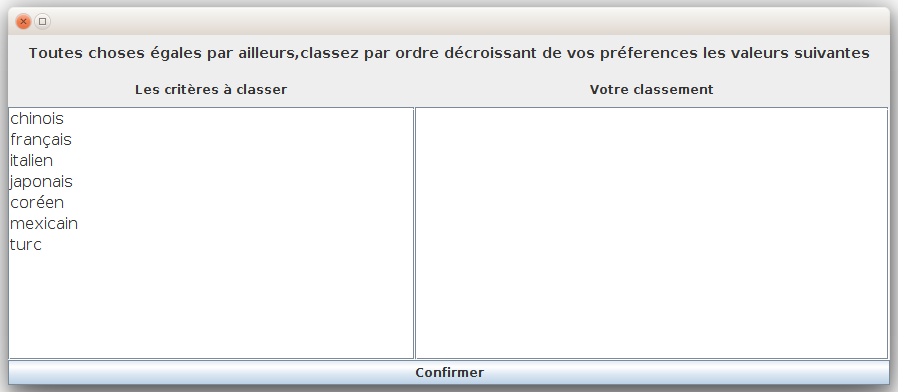
\includegraphics[width=4in]{Figures/pref.png}
%				\caption{\label{fig:pref} Interface for entering an order of preference. Example for the cuisine criteria}
%			\end{figure} 
			
			
		\subsubsection{Operational hypotheses}
		We therefore formulate the following operational hypotheses:
		\begin{itemize}
			\item \textit{\textbf{H1}}: The complementary and similar behaviors of virtual agents are perceived by participants.
				
				\subitem $\circ$ The behaviors of dominance attributed by participants to agents are \textit{significantly different} from those they have attributed to them selves.
				\subitem $\circ$ The behaviors of dominance attributed by the participants to the agents are \textit{similar} to the those they have attributed to them selves.
				
				\item \textit{ \textbf{H2}}: Negotiators achieve a greater common gain when negotiators establish a complementary dominance relationship.
					\subitem $\circ$ The restaurant chosen at the end of the negotiation has a satisfaction value which is significantly more important for the preferences of both negotiators in the complementary condition compared to the other conditions. 
					
					\item[$\bullet$] \textit{\textbf{H3}}: Negotiation converges more quickly when negotiators have a complementary dominance relationship.
						\subitem $\circ$ Participants will engage in more rounds of negotiations to find a compromise in the similar and neutral condition compared to the complementary condition.
						
					\item \textit{\textbf{H4}}: The participant feels more comfortable with a partner who expresses complementary behaviors of dominance.
						\subitem $\circ$ The perceived \emph{comfort} scores are higher for the complementary agent and control than for the similar agent.
						\subitem $\circ$ Participants find it easier to negotiate with the complementary agent than with other agents.
						
					\item \textit{\textbf{H5}}: Complementarity in the dominance relationship increases appreciation between negotiators.
						\subitem $\circ$ Participants will perceive the complementary agent as significantly more pleasant than the similar or neutral agent.
								
		\end{itemize}
		
		
	\section{Results}
	\label{sec:res}
	We conducted an intra-subject study in which 63 participants took part. However, two participants were excluded because they did not meet the required conditions (incorrect answers to the majority of the manipulation check questions).
	Therefore, our statistical study was conducted on the remaining 61 participants. 
	
		\subsection{Evaluation of the agent's behaviors}
			To study the differences between the behaviors of dominance expressed by agents and participants, non-parametric statistics were used because the normality of the data could not be ensured. For the main analysis, the Wilcoxon signed rank test was applied to assess each of the four behaviors.
			\begin{table*}[t]
				\caption{Difference in perception of dominance between the agent and the participant for each behavior} 
				\centering
				
				\begin{tabular}{p{1.5cm}  p{2.2cm}  p{1.5cm}  p{1.5cm}  p{1.5cm}  p{1.5cm}  p{1.5cm}}
					\hline\hline
					\textbf{Agent}& Evaluation & \textbf{D1} & \textbf{D2} & \textbf{D3} & \textbf{D4} \\ 
					\hline
					
					\multirow{3}{*} {\textbf{Comp.}}  &  Z-Wilcoxon  & -4.61 & -5.3 & -6.28 & -0.43 \\ 	
					& p-value & 2.88E-06 & 7.31E-08 & 1.42E-10 & \textbf{0.65 }\\ 
					& Effect size & -0.29 & -0.34 & -0.4 & -0.03\\ 
					\hline
					
					\multirow{3}{*} {\textbf{Similar}}  &  Z-Wilcoxon  & -1.57 & -2.21 & -1.45 & -1.33\\ 	
					& p-value & 0.11 & \textbf{0.024} & 0.14 & 0.17 \\ 
					& Effect size & -0.1 & -0.14& -0.09 & -0.08 \\ 
					\hline
					
					\multirow{3}{*} {\textbf{Neutral}}  &  Z-Wilcoxon  & -6.23 & -5.72 & -7.056 & -0.77\\ 	
					& p value & 2.52E-10 & 6.85E-09 & 8.19E-13 & \textbf{0.4351} \\ 
					& Effect size & -0.4 & -0.36 & -0.45 & -0.049 \\ 
					\hline \hline
					
				\end{tabular}
				
				\label{tab:domPercption}
			\end{table*}
			
	\subsubsection{Perception of complementarity of dominance}
	
	At the end of each negotiation, we asked participants to report on their behaviors of dominance expressed during the negotiation. For each dimension, we compared participants' perceptions of their behaviors with those expressed by the complementary agent. The descriptive statistics are presented in figure \ref{fig:comp}.
	
	
	The results of Wilcoxon's analysis revealed that participants perceived a significant difference between their behaviors and those of the agent as presented in the table \ref{tab:domPercption}. This difference concerns the behaviors \textbf{D1, D2} and \textbf{D3}. However, no significant differences were perceived for leadership behavior in negotiation \textbf{D4}.
	
		\begin{figure}[h]
			\centering
			% this is wide enough
			\subfloat [Perception score of dominance behaviors]{
				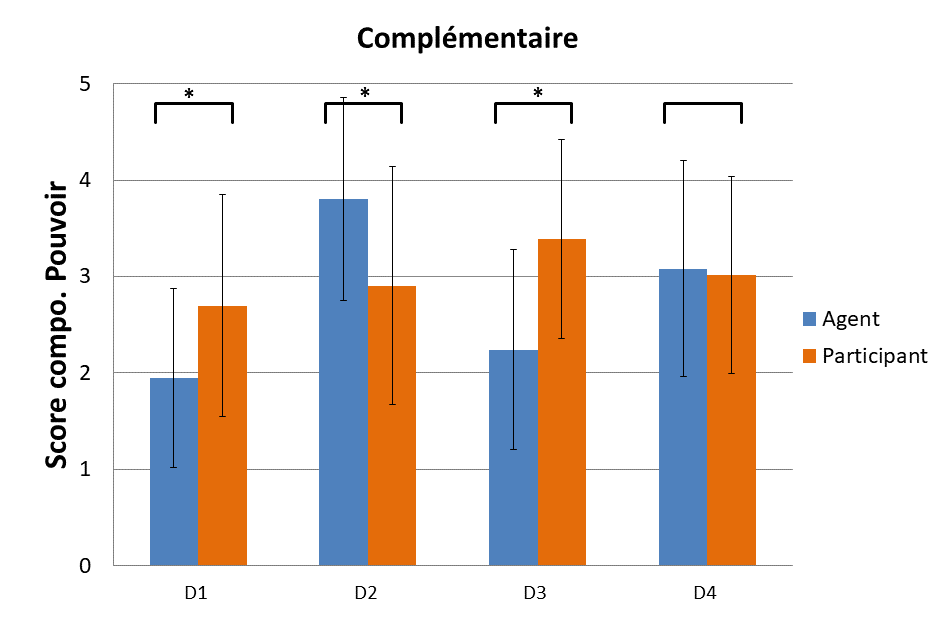
\includegraphics[clip=false,width=0.9\columnwidth]{figs/comPow.PNG}
			}
			
			% this has a too narrow subfigure
			\subfloat[Mean and standard deviation for the behavior of dominance perceived]{
				\begin{tabular}{l c c c c c c}
					\hline\hline
					\textbf{Agent} & Evaluation&  \textbf{D1} & \textbf{D2} & \textbf{D3} & \textbf{D4} \\
					\hline
					
					\multirow{2}{*}{\textbf{Comp.} }& Mean & 1,94& 3,80 & 2,24 & 3,08 \\
					& SD & 0,93 & 1,05 & 1,03 & 1,11 \\
					
					\hline
					\multirow{2}{*}{\textbf{Part.}}& Mean & 2,69 & 2,94 & 3,4 & 3,02 \\
					& SD & 1,14 & 1,23 & 1,03 & 1,02\\
					\hline
					\hline
				\end{tabular}
			}
			\caption{Perception of behaviors of dominance  with the complementary agent Bob}
			\label{fig:comp}
		\end{figure}
		
		\subsubsection{Perception of similarity of dominance}
		
		We also analyzed the negotiators' behaviors during their interactions with Agent Arthur. Descriptive statistics have already shown a strong similarity in the perception of all behaviors (see figure \ref{fig:sim}). We completed the study with a comparison of Wilcoxon which confirmed the absence of significant difference between the agent Arthur and  participants behaviors of dominance as presented in the table \ref{tab:domPercption}.  
		
			\begin{figure}[!tb]
				\centering
				% this is wide enough
				\subfloat[Perception score of dominance behaviors]{
					\centering
					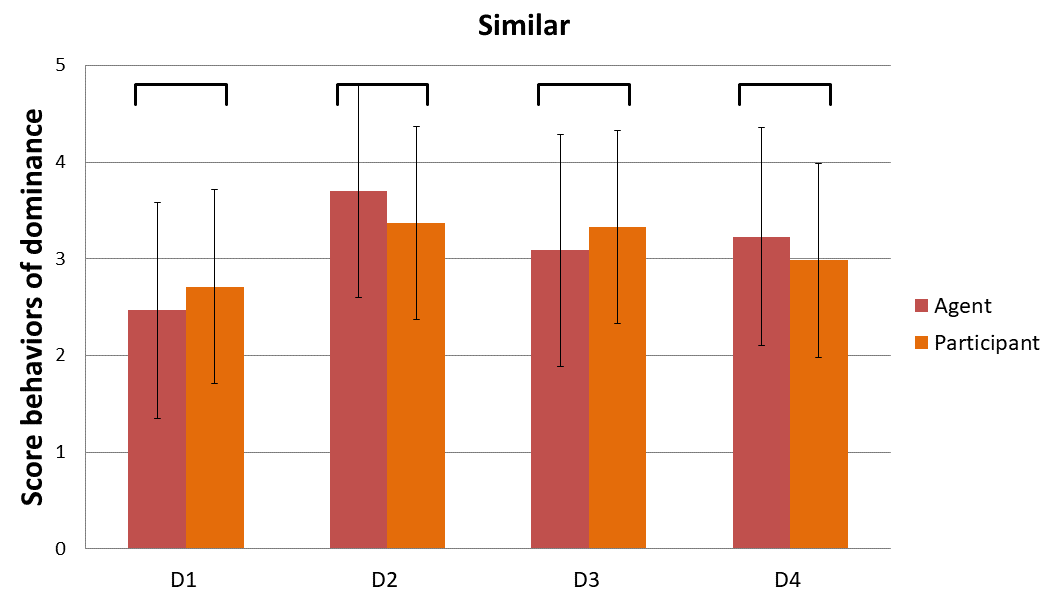
\includegraphics[clip=false]{Figures/chap7/simPow.PNG}
				}
				
				%\vspace{1em}
				% this has a too narrow subfigure
				\subfloat[Mean and standard deviation for the behavior of dominance perceived]{
					\centering
					\begin{tabular}{l c c c c c c}
						\hline\hline
						\textbf{Agent} & Evaluation& \textbf{D1} & \textbf{D2} & \textbf{D3} & \textbf{D4} \\
						\hline
						
						\multirow{2}{*}{\textbf{Simil.}}& Mean & 2,47 & 3,70 & 3,09 & 3,23 \\
						& SD & 1,11 & 1,10 & 1,19 & 1,12 \\
						
						\hline
						\multirow{2}{*}{\textbf{Part.}}& Mean & 2,71 & 3,37 & 3,33 & 2,98 \\
						& SD & 1,06 & 1,03 & 1,06 & 1,09\\
						\hline \hline
						
					\end{tabular}
				}
				\caption{Perception of behaviors of dominance  with the similar agent Arthur}
				\label{fig:sim}
			\end{figure}
			
		\subsubsection{Behaviors of the neutral agent}
		
		We conducted the same statistical studies to analyze the perception of the neutral agent's behaviors. The descriptive analysis presented in Figure \ref{fig:neutral} shows that participants perceived that the agent was adopting a complementary strategy for the behaviors \textbf{D1}, \textbf{D2} and \textbf{D3}. However, no significant differences were perceived for the \textbf{D4} behavior.
		
			\begin{figure}[!tb]
				\centering
				% this is wide enough
				\subfloat[Score de perception des comportements de dominance]{
					
					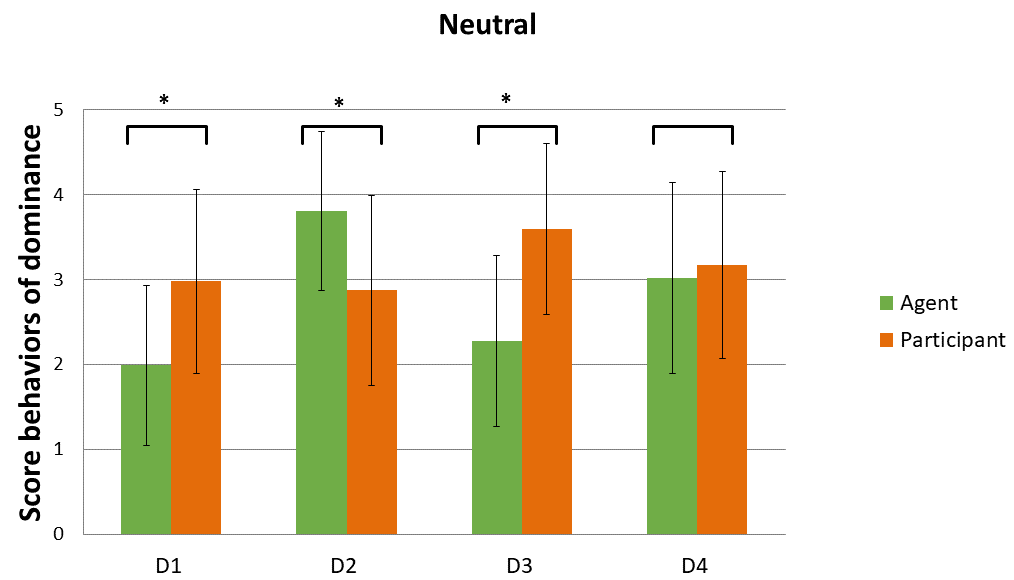
\includegraphics[clip=false]{Figures/chap7/neutrePow.PNG}
				}
				
				%\vspace{1em}
				% this has a too narrow subfigure
				\subfloat[Moyenne et écart type dans les comportements de dominance]{
					
					\begin{tabular}{l c c c c c c}
						\hline\hline
						\textbf{Agent} & Evaluation& \textbf{D1} & \textbf{D2} & \textbf{D3} & \textbf{D4} \\
						\hline
						
						\multirow{2}{*}{\textbf{Neutre}}& Moyenne & 1,99 & 3,81 & 2,28 & 3,02 \\
						& Ecart-type & 0,94 & 0,94 & 1,01 & 1,12 \\
						
						\hline
						\multirow{2}{*}{\textbf{Part}}& Moyenne & 2,98 & 2,88 & 3,60 & 3,17 \\
						
						& Ecart-type & 1,08 & 1,12 & 1,01 & 1,10 \\
						\hline \hline
						
					\end{tabular}
					
				}
				\caption{Perception des comportements de dominance avec l'agent neutre}
				\label{fig:neutre}
			\end{figure}
		
%----------------------------------------------------------------------------------------
					
			
%----------------------------------------------------------------------------------------
%	BIBLIOGRAPHY
%----------------------------------------------------------------------------------------

\printbibliography[title={Bibliography}] % Print the bibliography, section title in curly brackets

%----------------------------------------------------------------------------------------



\end{document}
